\chapter{Análisis del problema}

\section{Implicados}

En esta sección vamos a centrarnos en los implicados del problema a resolver ya que estos serán los usuarios finales de
la aplicación. Definiremos a continuación los distintos tipos de usuario:

\subsection{Tipos de usuario}

Los usuarios potenciales de la aplicación son:

\begin{itemize}
    \item Super-Administrador. Su función es gestionar la totalidad del aplicativo, teniendo acceso total a los datos
    almacenados por cada uno de los negocios. Podrá monitorizar el correcto funcionamiento de la aplicación y realizar
    correcciones o registrar incidencias si es necesario.

    \item Administrador. Su función es gestionar los datos de un negocio. En este caso existiría un usuario
    administrador por negocio y este tendrá acceso a los datos del mismo. Si detecta posibles errores también
    podrá registrar incidencias.

    \item Usuarios. Podrán consultar y reservar citas, así realizar pedidos en la tienda online.
    Además tendrán acceso a todos su datos como histórico de citas o histórico de pedidos.
\end{itemize}

\subsection{Resumen de implicados}

\begin{table}[H]
\begin{tabular}{|c|l|c|l|}
\hline
\textbf{Nombre} & \multicolumn{1}{c|}{\textbf{Descripción}} & \textbf{Tipo} & \multicolumn{1}{c|}{\textbf{Responsabilidad}} \\ \hline
Super-Administrador & \begin{tabular}[c]{@{}l@{}}Administrador \\ del sistema\end{tabular} & \begin{tabular}[c]{@{}c@{}}Usuario\\ producto\end{tabular} & \begin{tabular}[c]{@{}l@{}}Gestionar el sistema, moniro- \\ rizar sistema, gestionar inci- \\ dencias.\end{tabular} \\ \hline
Administrador & \begin{tabular}[c]{@{}l@{}}Administrador \\ del negocio\end{tabular} & \begin{tabular}[c]{@{}c@{}}Usuario\\ producto\end{tabular} & \begin{tabular}[c]{@{}l@{}}Gestionar el negocio, modificar \\ datos del negocio (citas, \\ productos,...), registrar \\ incidencias.\end{tabular} \\ \hline
Usuario & \begin{tabular}[c]{@{}l@{}}Cliente que \\ usa el sistema \\ de manera \\ convencional.\end{tabular} & \begin{tabular}[c]{@{}c@{}}Usuario\\ producto\end{tabular} & \begin{tabular}[c]{@{}l@{}}Reservar/modificar/cancelar \\ citas, realizar pedidos, \\ gestionar perfil de usuario.\end{tabular} \\ \hline
\end{tabular}
\caption{Resumen de implicados}
\end{table}

\subsection{Perfiles de los implicados}

\textbf{Administrador}

\begin{table}[H]
\begin{tabular}{|l|l|}
\hline
\textbf{Representante} & Nombre Apellidos \\ \hline
\textbf{Descripción} & Super-Administrador \\ \hline
\textbf{Tipo} & \begin{tabular}[c]{@{}l@{}}
Encargado del sistema completo, con responsabilidades\\ de gestión sobre el mismo.
\end{tabular} \\ \hline
\textbf{Responsabilidades} & \begin{tabular}[c]{@{}l@{}}
Gestionar el sistema correctamente: supervisar\\ los errores que puedan surgir en el aplicativo y controlar\\
el funcionamiento.
\end{tabular} \\ \hline
\textbf{Criterios de éxito} & \begin{tabular}[c]{@{}l@{}}
Que el sistema funcione adecuadamente con los pará-\\ metros óptimos y no exista información incorrecta.
\end{tabular} \\ \hline
\textbf{Implicación} &
Total, pues es el encargado principal del sistema. \\ \hline
\end{tabular}
\caption{Perfil de implicado: Super-Administrador}
\end{table}

\textbf{Trabajador}

\begin{table}[H]
\begin{tabular}{|l|l|}
\hline
\textbf{Representante} & Nombre Apellidos \\ \hline
\textbf{Descripción} & Administrador de negocio \\ \hline
\textbf{Tipo} & \begin{tabular}[c]{@{}l@{}}
Encargado del negocio al que pertenece, \\
con responsabilidades de gestión sobre el mismo.
\end{tabular} \\ \hline
\textbf{Responsabilidades} & \begin{tabular}[c]{@{}l@{}}
Gestionar su negocio: supervisar\\ y controlar los datos referentes a su negocio\\ para que no aparezcan incongruencias.
\end{tabular} \\ \hline
\textbf{Criterios de éxito} & \begin{tabular}[c]{@{}l@{}}
Que no se detecten errores en los datos almacenados.
\end{tabular} \\ \hline
\textbf{Implicación} &
Total a nivel de negocio. \\ \hline
\end{tabular}
\caption{Perfil de implicado: Trabajador}
\end{table}

\textbf{Cliente}

\begin{table}[H]
\begin{tabular}{|l|l|}
\hline
\textbf{Representante} & Nombre Apellidos \\ \hline
\textbf{Descripción} & Cliente de un negocio \\ \hline
\textbf{Tipo} & \begin{tabular}[c]{@{}l@{}}
Hace uso del aplicativo\\ Front-End sin tener\\ conocimiento inicial de uso.
\end{tabular} \\ \hline
\textbf{Responsabilidades} & \begin{tabular}[c]{@{}l@{}}
Crear su cuenta de usuario.\\
Reservar citas.\\
Realizar pedidos.\\
Gestionar su perfil de usuario.\\
\end{tabular} \\ \hline
\textbf{Criterios de éxito} & \begin{tabular}[c]{@{}l@{}}
Poder realizar sus\\ responsabilidades sin errores\\ y de forma sencilla.
\end{tabular} \\ \hline
\textbf{Implicación} &
Total a nivel de negocio. Sin clientes no hay negocio.\\ \hline
\end{tabular}
\caption{Perfil de implicado: Cliente}
\end{table}

\section{Especificación de requisitos}

\subsection{Requisitos funcionales}

Desarrollaremos aquí los requisitos funcionales para la definición de funcionalidades del sistema de software.

\begin{enumerate}[leftmargin=1.75cm,start=1,label={\bfseries RF-\arabic*.}]
\setlength\itemsep{1em} % Aumenta el interlineado entre ítems
    \item \textbf{Gestión de super-administradores.} Se permitirá el alta/baja con el rol de super-administrador del
    sistema. Podrá acceder a todos los datos almacenados en este.
    \begin{enumerate}[start=1,label={\bfseries RF-1.\arabic*.}]
        \item \textbf{Alta de super-administrador.} Se dará de alta a cada super-administrador con sus datos personales.
        \item \textbf{Baja de super-administrador.} Se dará de baja al super-administrador y la información relativa a
        él será eliminada. Siempre deberá haber un usuario de este rol para las revisiones tecnicas del aplicativo.
        \item \textbf{Consultar datos del sistema.} Se podrán consultar todos los datos almacenados en el sistema.
        \item \textbf{Modificar datos del sistema.} Se podrán modificar todos los datos almacenados en el sistema.
    \end{enumerate}

    \item \textbf{Gestión de trabajadores.} Se permitirá el alta/baja con el rol de trabajador de negocio,
    así como consultar y modificar sus datos. También podrá acceder a los datos de los clientes dados de alta
    en el mismo negocio.
    \begin{enumerate}[start=1,label={\bfseries RF-2.\arabic*.}]
        \item \textbf{Alta de trabajador.} Se dará de alta a cada trabajador con sus datos personales.
        \item \textbf{Baja de trabajador.} Se dará de baja al trabajador y la información relativa a él será eliminada.
        \item \textbf{Consultar datos de trabajador.} Se podrá consultar los datos relativos a un determinado
        trabajador (datos personales, citas asignadas, etc.).
        \item \textbf{Modificar datos de trabajador.} Se podrán modificar modificar los datos personales de un
        trabajador.
        \item \textbf{Consultar citas de trabajador.} Se podrá consultar los citas previas asignadas al trabajador.
    \end{enumerate}

    \item \textbf{Gestión de clientes.} Se permitirá el alta/baja con el rol de usuario del negocio,
    así como consultar y modificar sus datos.
    \begin{enumerate}[start=1,label={\bfseries RF-3.\arabic*.}]
        \item \textbf{Alta de cliente.} Un cliente potencial se podrá dar de alta en un negocio determinado.
        \item \textbf{Baja de cliente.} Un cliente se podrá dar de baja de un negocio determinado.
        \item \textbf{Consultar datos de cliente.} Un cliente podrá consultar sus datos de un respectivo negocio.
        \item \textbf{Modificar datos de cliente.} Un cliente podrá modificar sus datos personales con los que se ha
        registrado en un negocio.
        \item \textbf{Consultar citas de trabajador.} Un cliente podrá consultar su historial de citas previas
        reservadas.
    \end{enumerate}

    \item \textbf{Gestión de citas previas.} Se permitirá realizar reservas o cancelaciones de citas previas así como
    acceder a un histórico de estas según el tipo de usuario.
    \begin{enumerate}[start=1,label={\bfseries RF-4.\arabic*.}]
        \item \textbf{Reserva de cita previa por cliente.} Una cita previa podrá ser reservada por un cliente siempre
        que la fecha sea válida y haya trabajadores disponibles en el negocio.
        \item \textbf{Cancelación de cita previa por cliente.} Una cita previa podrá ser cancelada por un cliente
        siempre que esté pendiente.
        \item \textbf{Reserva de cita previa por trabajador.} Una cita previa podrá ser reservada por un trabajador
        siempre que la fecha sea válida, el trabajador pueda atenderla y el cliente no tenga una cita ya pendiente.
        \item \textbf{Cancelación de cita previa por cliente.} Una cita previa podrá ser cancelada por un trabajador
        siempre que la cita a cancelar esté asignada a él y esté en estado pendiente.\\
    \end{enumerate}

    \item \textbf{Gestión de productos.} Se permitirá realizar gestiones sobre los productos de la tienda para su venta online.
    \begin{enumerate}[start=1,label={\bfseries RF-5.\arabic*.}]
        \item \textbf{Alta de producto.} Un producto podrá ser dado de alta por un trabajador de un negocio o por un super-administrador.
        \item \textbf{Baja de producto.} Un producto podrá ser dado de baja por un trabajador de un negocio o por un super-administrador.
        \item \textbf{Modificación de información de producto.} La informació de un producto podrá ser modificado por un trabajador de un negocio o por un super-administrador.
    \end{enumerate}
    
    \item \textbf{Gestión de pedidos.} Se permitirá realizar pedidos online de productos ofertados por el propio negocio así como acceder al historial y estado de los pedidos.
    \begin{enumerate}[start=1,label={\bfseries RF-6.\arabic*.}]
        \item \textbf{Realización de pedido.} Un pedido podrá ser realizado por un usuario del sistema de productos disponibles en la tienda web ofrecidos por el negocio.
        \item \textbf{Cancelación de pedido.} Un pedido podrá ser cancelado por un usuario del sistema siempre y cuando pertenezca al propio usuario mismo y siga en un estado pendiente.
        \item \textbf{Seguimiento de pedido.} Un pedido podrá ser seguido por un usuario del sistema siempre y cuando pertenezca al propio usuario mismo. Podrá ver los estados por los que ha ido pasando en el tiempo (pendiente, en preparación, enviado, entregado, etc), además de poder ver un resumen del mismo.
    \end{enumerate}
\end{enumerate}

\subsection{Requisitos de información}

Requisitos de información, describen la información que debe almacenar y gestionar el sistema para dar soporte a los
procesos de negocio.

\begin{enumerate}[leftmargin=1.6cm,start=1,label={\bfseries RI-\arabic*.}]
\setlength\itemsep{1em} % Aumenta el interlineado entre ítems
    \item \textbf{Administrador}
    \\\textbf{Contenido:} email, nombre, apellidos, contraseña, número de teléfono, dirección y fecha de creación.
	\\\textbf{Requisitos asociados:} RF-1

	\item \textbf{Trabajador}
    \\\textbf{Contenido:} email, nombre, apellidos, contraseña, número de teléfono, dirección y fecha de creación.
    \\\textbf{Requisitos asociados:} RF-2.1, RF-2.2, RF-2.3, RF-2.4

    \item \textbf{Cliente}
    \\\textbf{Contenido:} email, nombre, apellidos, contraseña, número de teléfono, dirección y fecha de creación.
    \\\textbf{Requisitos asociados:} RF-3.1, RF-3.2, RF-3.3, RF-3.4

    \item \textbf{Citas}
    \\\textbf{Contenido:} trabajador, cliente, fecha de reserva.
    \\\textbf{Requisitos asociados:} RF-4, RF-2.5, RF-3.5\\
    
    \item \textbf{Producto}
    \\\textbf{Contenido:} nombre, descripción, categoria, stock, precio, fecha de creación.
    \\\textbf{Requisitos asociados:} RF-5 RF-6.1\\
    
    \item \textbf{Pedido}
    \\\textbf{Contenido:} cliente, dirección de envio, fecha de pedido, productos, estado, importe total.
    \\\textbf{Requisitos asociados:} RF-6\\
\end{enumerate}

\subsection{Restricciones semánticas}

Restricciones aplicadas a los requisitos funcionales y a los requisitos de información
para su correcto uso y almacenamiento.

\begin{enumerate}[leftmargin=1.75cm,start=1,label={\bfseries RS-\arabic*.}]
\setlength\itemsep{1em} % Aumenta el interlineado entre ítems

    \item \textbf{Alta super-administrador.} En el formulario de alta de super-administrador deberá comprobarse:
    \begin{enumerate}[start=1,label={\bfseries RS-1.\arabic*.}]
        \item \textbf{Email:} debe tener un formato válido.
        \item \textbf{Nombre:} no puede ser nulo o estar vacío.
        \item \textbf{Apellidos:} no puede ser nulo o estar vacío.
        \item \textbf{Número de teléfono:} debe ser un número válido.
        \item \textbf{Contraseña:} alfanumérica de más de 8 caracteres.
        \item \textbf{Dirección:} puede ser nulo hasta el momento de la realización de un pedido.
    \end{enumerate}

    \item \textbf{Alta de trabajador.} En el formulario de alta de trabajador deberá comprobarse:
    \begin{enumerate}[start=1,label={\bfseries RS-2.\arabic*.}]
        \item \textbf{Email:} debe tener un formato válido.
        \item \textbf{Nombre:} no puede ser nulo o estar vacío.
        \item \textbf{Apellidos:} no puede ser nulo o estar vacío.
        \item \textbf{Número de teléfono:} debe ser un número válido.
        \item \textbf{Contraseña:} alfanumérica de más de 8 caracteres.
        \item \textbf{Dirección:} puede ser nulo hasta el momento de la realización de un pedido.
    \end{enumerate}

    \item \textbf{Alta de cliente.} En el formulario de alta de cliente deberá comprobarse:
    \begin{enumerate}[start=1,label={\bfseries RS-3.\arabic*.}]
        \item \textbf{Email:} debe tener un formato válido.
        \item \textbf{Nombre:} no puede ser nulo o estar vacío.
        \item \textbf{Apellidos:} no puede ser nulo o estar vacío.
        \item \textbf{Número de teléfono:} debe ser un número válido.
        \item \textbf{Contraseña:} alfanumérica de más de 8 caracteres.
        \item \textbf{Dirección:} puede ser nulo hasta el momento de la realización de un pedido.
    \end{enumerate}

    \item \textbf{Reserva de cita previa por cliente.} Habrá varias restricciones para realizar la reserva de citas
    \begin{enumerate}[start=1,label={\bfseries RS-4.\arabic*.}]
        \item \textbf{Fecha válida:} la fecha está en horario de trabajo.
        \item \textbf{Trabajador disponible:} hay un trabajador disponible para atender la cita a la fecha indicada.
        \item \textbf{No existen citas pendientes:} el cliente no tiene ya una cita previa pendiente.
    \end{enumerate}

    \item \textbf{Reserva de cita previa por trabajador.} Habrá varias restricciones para realizar la reserva de citas
    \begin{enumerate}[start=1,label={\bfseries RS-5.\arabic*.}]
        \item \textbf{Fecha válida:} la fecha está en horario de trabajo.
        \item \textbf{Trabajador disponible:} el trabajador debe estar disponible para atender la cita.
        \item \textbf{Cliente:} deberá indicarse un cliente existente para la cita.
        \item \textbf{No existen citas pendientes:} el cliente no tiene ya una cita previa pendiente.
    \end{enumerate}
    
    \item \textbf{Alta de producto.} En el formulario de alta de producto deberá comprobarse:
    \begin{enumerate}[start=1,label={\bfseries RS-6.\arabic*.}]
        \item \textbf{Nombre:} no puede ser nulo o estar vacío.
        \item \textbf{Descripción:} no puede ser nulo o estar vacío.
        \item \textbf{Categoría:} no puede ser nulo o estar vacío.
        \item \textbf{Stock:} debe de ser un entero mayor o igual a cero.
        \item \textbf{Precio:} debe ser un número con decimales mayor o igual a cero.
    \end{enumerate}
    
    \item \textbf{Realización de pedido.} En el formulario de alta de producto deberá comprobarse:
    \begin{enumerate}[start=1,label={\bfseries RS-7.\arabic*.}]
        \item \textbf{Dirección de envio:} no puede ser nulo o estar vacío.
        \item \textbf{Productos:} no puede ser nulo o estar vacio.
    \end{enumerate}
\end{enumerate}

\subsection{Requisitos No Funcionales}

\section{Modelo de casos de uso}

\subsection{Diagramas de casos de uso}

Un diagrama de casos de uso es una forma de diagrama de comportamiento UML mejorado. Con estos representaremos
los procesos del sistema de negocio así como los procesos de programación orientada a objetos.\\

\begin{figure}[H]
    \centering
    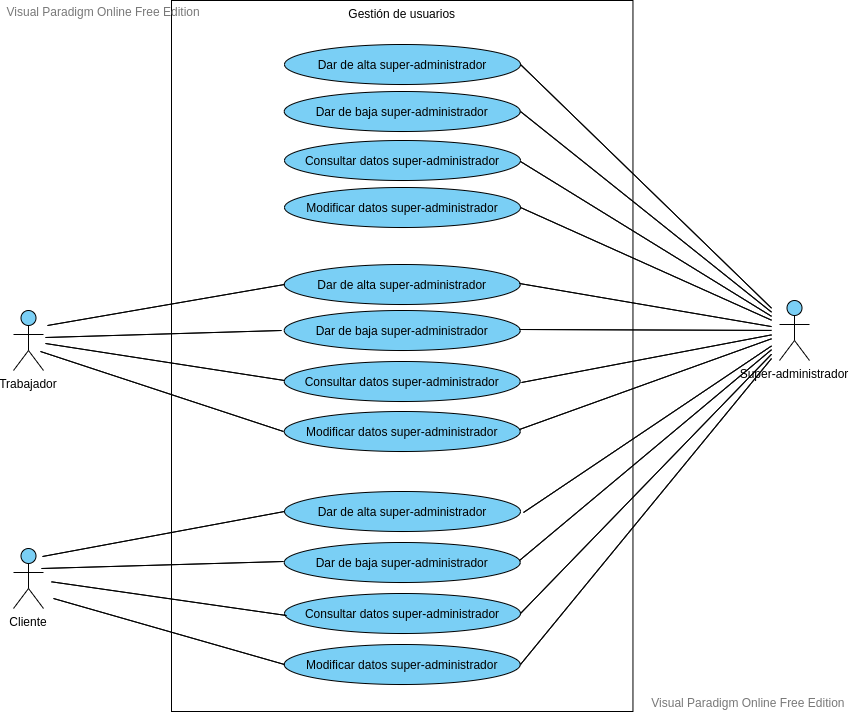
\includegraphics[width=0.9\textwidth]{images/Gestion_Usuarios.png}
    \caption{Diagrama de caso de uso - Gestión de usuarios}
    \label{CU1}
\end{figure}

\begin{figure}[H]
    \centering
    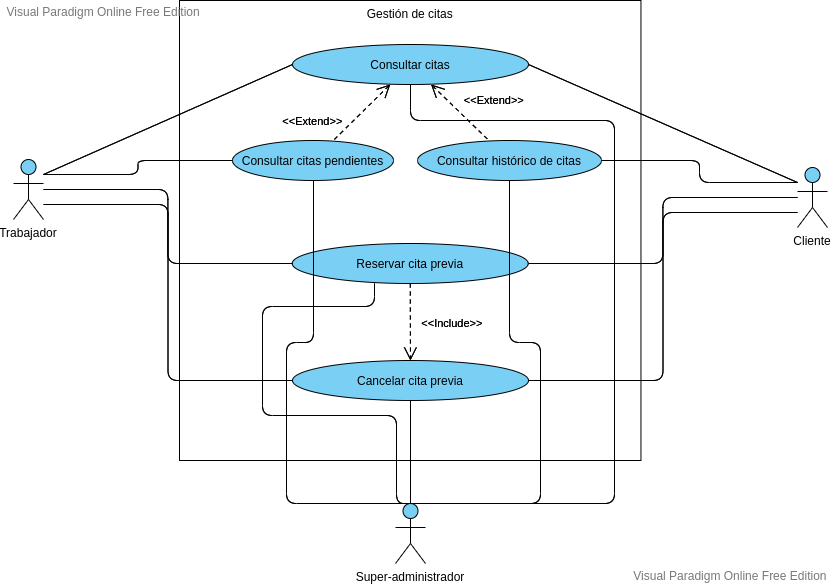
\includegraphics[width=0.9\textwidth]{images/Gestion_Citas.png}
    \caption{Diagrama de caso de uso - Gestión de citas}
    \label{CU1}
\end{figure}

\begin{figure}[H]
    \centering
    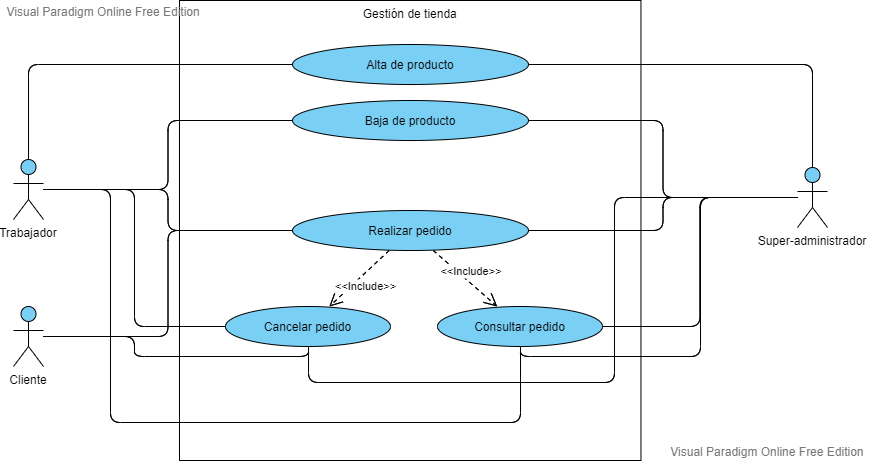
\includegraphics[width=0.9\textwidth]{images/Gestion_Tienda.png}
    \caption{Diagrama de caso de uso - Gestión de tienda}
    \label{CU1}
\end{figure}

\subsection{Descripción de los casos de uso}

En las siguientes tablas se detallan los casos de uso definidos en el apartado anterior. Podemos ver información sobre
los actores que interactuan en ella, el tipo, los requisitos funcionales incluidos, las precondiciones y
poscondiciones relativas a este y el propósito que cumple, además de un breve resumen que describe a un más alto
nivel lo que proporciona el caso de uso.

Los diferentes tipos de casos de uso son:

\begin{itemize}
    \item Según su importancia:
    \begin{itemize}
        \item Primarios: Procesos comunes más importantes.
        \item Secundarios: Procesos menores o raros.
        \item Opcionales: Procesos que pueden no abordarse.
    \end{itemize}

    \item Según el nivel de detalle
    \begin{itemize}
        \item Alto nivel: Descripción general del procesamiento.
        \item Extendidos: Descripción de la secuencia de acción completa entre actores y sistema.
    \end{itemize}

    \item Según el nivel de abstracción
    \begin{itemize}
        \item Esencial: Expresado de forma abstracta, contiene poca tecnología y pocos detalles de diseño.
        \item Real: Expresado en base al diseño actual, en el que aparecen relaciones con la interfaz de usuario.
    \end{itemize}
\end{itemize}

% SUPER-ADMINISTRADOR

\begin{table}[H]
\begin{tabular}{lll}
\hline
\rowcolor[HTML]{EFEFEF}
\multicolumn{1}{|l|}{\cellcolor[HTML]{EFEFEF}\textbf{Caso de uso}} & \multicolumn{1}{l|}{\cellcolor[HTML]{EFEFEF}
    Dar de alta super-administrador
} & \multicolumn{1}{l|}{\cellcolor[HTML]{EFEFEF}
    CU-1
} \\ \hline
\multicolumn{1}{|l|}{\textbf{Actores}} & \multicolumn{2}{l|}{
    Super-administrador
} \\ \hline
\multicolumn{1}{|l|}{\textbf{Tipo}} & \multicolumn{2}{l|}{
    Primario, básico y esencial
} \\ \hline
\multicolumn{1}{|l|}{\textbf{Referencias}} & \multicolumn{2}{l|}{
    RF-1.1
} \\ \hline
\multicolumn{1}{|l|}{\textbf{Precondición}} & \multicolumn{2}{l|}{\begin{tabular}[c]{@{}l@{}}
    Debe existir previamente un super-administrador que pueda \\ llevar a cabo esta función. Si no hay ninguno \\
    deberá añadirse por base de datos
\end{tabular}} \\ \hline
\multicolumn{1}{|l|}{\textbf{Poscondición}} & \multicolumn{2}{l|}{
    El super-administrador quedará registrado en el sistema
} \\ \hline
\multicolumn{3}{l}{} \\ \hline
\rowcolor[HTML]{EFEFEF}
\multicolumn{3}{|l|}{\cellcolor[HTML]{EFEFEF}\textbf{Propósito}} \\ \hline
\multicolumn{3}{|l|}{
    Dar de alta un nuevo super-administrador en el sistema
} \\ \hline
\multicolumn{3}{l}{} \\ \hline
\rowcolor[HTML]{EFEFEF}
\multicolumn{3}{|l|}{\cellcolor[HTML]{EFEFEF}\textbf{Resumen}} \\ \hline
\multicolumn{3}{|l|}{\begin{tabular}[c]{@{}l@{}}
    Se darán de alta usuarios con rol super-administrador, los cuales podrán \\ encargarse de la supervisión
    del sistema
\end{tabular}} \\ \hline
\end{tabular}
\end{table}

\begin{table}[H]
\begin{tabular}{lll}
\hline
\rowcolor[HTML]{EFEFEF}
\multicolumn{1}{|l|}{\cellcolor[HTML]{EFEFEF}\textbf{Caso de uso}} & \multicolumn{1}{l|}{\cellcolor[HTML]{EFEFEF}
    Dar de baja super-administrador
} & \multicolumn{1}{l|}{\cellcolor[HTML]{EFEFEF}
    CU-2
} \\ \hline
\multicolumn{1}{|l|}{\textbf{Actores}} & \multicolumn{2}{l|}{
    Super-administrador
} \\ \hline
\multicolumn{1}{|l|}{\textbf{Tipo}} & \multicolumn{2}{l|}{
    Primario, básico y esencial
} \\ \hline
\multicolumn{1}{|l|}{\textbf{Referencias}} & \multicolumn{2}{l|}{
    RF-1.2
} \\ \hline
\multicolumn{1}{|l|}{\textbf{Precondición}} & \multicolumn{2}{l|}{\begin{tabular}[c]{@{}l@{}}
    Debe existir previamente el super-administrador al que \\
    se quiera realizar la baja
\end{tabular}} \\ \hline
\multicolumn{1}{|l|}{\textbf{Poscondición}} & \multicolumn{2}{l|}{
    El super-administrador quedará eliminado del sistema
} \\ \hline
\multicolumn{3}{l}{} \\ \hline
\rowcolor[HTML]{EFEFEF}
\multicolumn{3}{|l|}{\cellcolor[HTML]{EFEFEF}\textbf{Propósito}} \\ \hline
\multicolumn{3}{|l|}{
    Dar de baja a un super-administrador del sistema
} \\ \hline
\multicolumn{3}{l}{} \\ \hline
\rowcolor[HTML]{EFEFEF}
\multicolumn{3}{|l|}{\cellcolor[HTML]{EFEFEF}\textbf{Resumen}} \\ \hline
\multicolumn{3}{|l|}{\begin{tabular}[c]{@{}l@{}}
    Se darán de baja a usuarios con rol super-administrador, eliminando \\
    su información de la base de datos del sistema
\end{tabular}} \\ \hline
\end{tabular}
\end{table}

\begin{table}[H]
\begin{tabular}{lll}
\hline
\rowcolor[HTML]{EFEFEF}
\multicolumn{1}{|l|}{\cellcolor[HTML]{EFEFEF}\textbf{Caso de uso}} & \multicolumn{1}{l|}{\cellcolor[HTML]{EFEFEF}
    Consultar datos del super-administrador
} & \multicolumn{1}{l|}{\cellcolor[HTML]{EFEFEF}
    CU-3
} \\ \hline
\multicolumn{1}{|l|}{\textbf{Actores}} & \multicolumn{2}{l|}{
    Super-administrador
} \\ \hline
\multicolumn{1}{|l|}{\textbf{Tipo}} & \multicolumn{2}{l|}{
    Primario, básico y esencial
} \\ \hline
\multicolumn{1}{|l|}{\textbf{Referencias}} & \multicolumn{2}{l|}{
    RF-1.3
} \\ \hline
\multicolumn{1}{|l|}{\textbf{Precondición}} & \multicolumn{2}{l|}{\begin{tabular}[c]{@{}l@{}}
    Debe existir previamente el super-administrador para \\
    poder consultar sus datos
\end{tabular}} \\ \hline
\multicolumn{1}{|l|}{\textbf{Poscondición}} & \multicolumn{2}{l|}{
    El super-administrador no sufrirá modificaciones
} \\ \hline
\multicolumn{3}{l}{} \\ \hline
\rowcolor[HTML]{EFEFEF}
\multicolumn{3}{|l|}{\cellcolor[HTML]{EFEFEF}\textbf{Propósito}} \\ \hline
\multicolumn{3}{|l|}{
    Consultar los datos personales como usuario super-administrador del sistema
} \\ \hline
\multicolumn{3}{l}{} \\ \hline
\rowcolor[HTML]{EFEFEF}
\multicolumn{3}{|l|}{\cellcolor[HTML]{EFEFEF}\textbf{Resumen}} \\ \hline
\multicolumn{3}{|l|}{\begin{tabular}[c]{@{}l@{}}
    Se podrá consultar los datos personales como usuario \\
    con rol super-administrador del sistema
\end{tabular}} \\ \hline
\end{tabular}
\end{table}

\begin{table}[H]
\begin{tabular}{lll}
\hline
\rowcolor[HTML]{EFEFEF}
\multicolumn{1}{|l|}{\cellcolor[HTML]{EFEFEF}\textbf{Caso de uso}} & \multicolumn{1}{l|}{\cellcolor[HTML]{EFEFEF}
    Modificar datos del super-administrador
} & \multicolumn{1}{l|}{\cellcolor[HTML]{EFEFEF}
    CU-4
} \\ \hline
\multicolumn{1}{|l|}{\textbf{Actores}} & \multicolumn{2}{l|}{
    Super-administrador
} \\ \hline
\multicolumn{1}{|l|}{\textbf{Tipo}} & \multicolumn{2}{l|}{
    Primario, básico y esencial
} \\ \hline
\multicolumn{1}{|l|}{\textbf{Referencias}} & \multicolumn{2}{l|}{
    RF-1.4
} \\ \hline
\multicolumn{1}{|l|}{\textbf{Precondición}} & \multicolumn{2}{l|}{\begin{tabular}[c]{@{}l@{}}
    Debe existir previamente el super-administrador para \\
    poder modificar sus datos personales
\end{tabular}} \\ \hline
\multicolumn{1}{|l|}{\textbf{Poscondición}} & \multicolumn{2}{l|}{
    Los datos del super-administrador sufrirán modificaciones
} \\ \hline
\multicolumn{3}{l}{} \\ \hline
\rowcolor[HTML]{EFEFEF}
\multicolumn{3}{|l|}{\cellcolor[HTML]{EFEFEF}\textbf{Propósito}} \\ \hline
\multicolumn{3}{|l|}{
    Modificar los datos personales como usuario super-administrador del sistema
} \\ \hline
\multicolumn{3}{l}{} \\ \hline
\rowcolor[HTML]{EFEFEF}
\multicolumn{3}{|l|}{\cellcolor[HTML]{EFEFEF}\textbf{Resumen}} \\ \hline
\multicolumn{3}{|l|}{\begin{tabular}[c]{@{}l@{}}
    Se podrán modificar los datos personales como usuario \\
    con rol super-administrador del sistema
\end{tabular}} \\ \hline
\end{tabular}
\end{table}

% TRABAJADORES

\begin{table}[H]
\begin{tabular}{lll}
\hline
\rowcolor[HTML]{EFEFEF}
\multicolumn{1}{|l|}{\cellcolor[HTML]{EFEFEF}\textbf{Caso de uso}} & \multicolumn{1}{l|}{\cellcolor[HTML]{EFEFEF}
    Dar de alta trabajador
} & \multicolumn{1}{l|}{\cellcolor[HTML]{EFEFEF}
    CU-5
} \\ \hline
\multicolumn{1}{|l|}{\textbf{Actores}} & \multicolumn{2}{l|}{
    Super-administrador y trabajador
} \\ \hline
\multicolumn{1}{|l|}{\textbf{Tipo}} & \multicolumn{2}{l|}{
    Primario, básico y esencial
} \\ \hline
\multicolumn{1}{|l|}{\textbf{Referencias}} & \multicolumn{2}{l|}{
    RF-2.1
} \\ \hline
\multicolumn{1}{|l|}{\textbf{Precondición}} & \multicolumn{2}{l|}{\begin{tabular}[c]{@{}l@{}}
    Debe existir previamente un super-administrador o \\
    un trabajador del negocio que pueda llevar a cabo \\
    esta función. Si no hay ninguno deberá añadirse \\
    por base de datos
\end{tabular}} \\ \hline
\multicolumn{1}{|l|}{\textbf{Poscondición}} & \multicolumn{2}{l|}{
    El trabajador quedará registrado en el sistema
} \\ \hline
\multicolumn{3}{l}{} \\ \hline
\rowcolor[HTML]{EFEFEF}
\multicolumn{3}{|l|}{\cellcolor[HTML]{EFEFEF}\textbf{Propósito}} \\ \hline
\multicolumn{3}{|l|}{
    Dar de alta un nuevo trabajador en el negocio
} \\ \hline
\multicolumn{3}{l}{} \\ \hline
\rowcolor[HTML]{EFEFEF}
\multicolumn{3}{|l|}{\cellcolor[HTML]{EFEFEF}\textbf{Resumen}} \\ \hline
\multicolumn{3}{|l|}{\begin{tabular}[c]{@{}l@{}}
    Se darán de alta usuarios con rol trabajador, los cuales podrán \\
    encargarse de la supervisión del negocio y atender citas
\end{tabular}} \\ \hline
\end{tabular}
\end{table}

\begin{table}[H]
\begin{tabular}{lll}
\hline
\rowcolor[HTML]{EFEFEF}
\multicolumn{1}{|l|}{\cellcolor[HTML]{EFEFEF}\textbf{Caso de uso}} & \multicolumn{1}{l|}{\cellcolor[HTML]{EFEFEF}
    Dar de baja trabajador
} & \multicolumn{1}{l|}{\cellcolor[HTML]{EFEFEF}
    CU-6
} \\ \hline
\multicolumn{1}{|l|}{\textbf{Actores}} & \multicolumn{2}{l|}{
    Super-administrador y trabajador
} \\ \hline
\multicolumn{1}{|l|}{\textbf{Tipo}} & \multicolumn{2}{l|}{
    Primario, básico y esencial
} \\ \hline
\multicolumn{1}{|l|}{\textbf{Referencias}} & \multicolumn{2}{l|}{
    RF-2.2
} \\ \hline
\multicolumn{1}{|l|}{\textbf{Precondición}} & \multicolumn{2}{l|}{\begin{tabular}[c]{@{}l@{}}
    Debe existir previamente el trabajador al que \\
    se quiera realizar la baja
\end{tabular}} \\ \hline
\multicolumn{1}{|l|}{\textbf{Poscondición}} & \multicolumn{2}{l|}{
    El trabajador quedará eliminado del sistema
} \\ \hline
\multicolumn{3}{l}{} \\ \hline
\rowcolor[HTML]{EFEFEF}
\multicolumn{3}{|l|}{\cellcolor[HTML]{EFEFEF}\textbf{Propósito}} \\ \hline
\multicolumn{3}{|l|}{
    Dar de baja a un trabajador del sistema
} \\ \hline
\multicolumn{3}{l}{} \\ \hline
\rowcolor[HTML]{EFEFEF}
\multicolumn{3}{|l|}{\cellcolor[HTML]{EFEFEF}\textbf{Resumen}} \\ \hline
\multicolumn{3}{|l|}{\begin{tabular}[c]{@{}l@{}}
    Se darán de baja a usuarios con rol trabajador, eliminando \\
    su información de la base de datos del sistema
\end{tabular}} \\ \hline
\end{tabular}
\end{table}

\begin{table}[H]
\begin{tabular}{lll}
\hline
\rowcolor[HTML]{EFEFEF}
\multicolumn{1}{|l|}{\cellcolor[HTML]{EFEFEF}\textbf{Caso de uso}} & \multicolumn{1}{l|}{\cellcolor[HTML]{EFEFEF}
    Consultar datos del trabajador
} & \multicolumn{1}{l|}{\cellcolor[HTML]{EFEFEF}
    CU-7
} \\ \hline
\multicolumn{1}{|l|}{\textbf{Actores}} & \multicolumn{2}{l|}{
    Super-administrador y trabajador
} \\ \hline
\multicolumn{1}{|l|}{\textbf{Tipo}} & \multicolumn{2}{l|}{
    Primario, básico y esencial
} \\ \hline
\multicolumn{1}{|l|}{\textbf{Referencias}} & \multicolumn{2}{l|}{
    RF-2.3
} \\ \hline
\multicolumn{1}{|l|}{\textbf{Precondición}} & \multicolumn{2}{l|}{\begin{tabular}[c]{@{}l@{}}
    Debe existir previamente el trabajador para \\
    poder consultar sus datos
\end{tabular}} \\ \hline
\multicolumn{1}{|l|}{\textbf{Poscondición}} & \multicolumn{2}{l|}{
    El trabajador no sufrirá modificaciones
} \\ \hline
\multicolumn{3}{l}{} \\ \hline
\rowcolor[HTML]{EFEFEF}
\multicolumn{3}{|l|}{\cellcolor[HTML]{EFEFEF}\textbf{Propósito}} \\ \hline
\multicolumn{3}{|l|}{\begin{tabular}[c]{@{}l@{}}{
    Consultar los datos personales como usuario trabajador del sistema \\
    de un negocio determinado
} \\ \hline
\end{tabular}} \\ \hline
\multicolumn{3}{l}{} \\ \hline
\rowcolor[HTML]{EFEFEF}
\multicolumn{3}{|l|}{\cellcolor[HTML]{EFEFEF}\textbf{Resumen}} \\ \hline
\multicolumn{3}{|l|}{\begin{tabular}[c]{@{}l@{}}
    Se podrá consultar los datos personales como usuario \\
    con rol trabajador del sistema de un negocio determinado
\end{tabular}} \\ \hline
\end{tabular}
\end{table}

\begin{table}[H]
\begin{tabular}{lll}
\hline
\rowcolor[HTML]{EFEFEF}
\multicolumn{1}{|l|}{\cellcolor[HTML]{EFEFEF}\textbf{Caso de uso}} & \multicolumn{1}{l|}{\cellcolor[HTML]{EFEFEF}
    Modificar datos del trabajador
} & \multicolumn{1}{l|}{\cellcolor[HTML]{EFEFEF}
    CU-8
} \\ \hline
\multicolumn{1}{|l|}{\textbf{Actores}} & \multicolumn{2}{l|}{
    Super-administrador y trabajador
} \\ \hline
\multicolumn{1}{|l|}{\textbf{Tipo}} & \multicolumn{2}{l|}{
    Primario, básico y esencial
} \\ \hline
\multicolumn{1}{|l|}{\textbf{Referencias}} & \multicolumn{2}{l|}{
    RF-2.4
} \\ \hline
\multicolumn{1}{|l|}{\textbf{Precondición}} & \multicolumn{2}{l|}{\begin{tabular}[c]{@{}l@{}}
    Debe existir previamente el trabajador para \\
    poder modificar sus datos personales
\end{tabular}} \\ \hline
\multicolumn{1}{|l|}{\textbf{Poscondición}} & \multicolumn{2}{l|}{
    Los datos del trabajador sufrirán modificaciones
} \\ \hline
\multicolumn{3}{l}{} \\ \hline
\rowcolor[HTML]{EFEFEF}
\multicolumn{3}{|l|}{\cellcolor[HTML]{EFEFEF}\textbf{Propósito}} \\ \hline
\multicolumn{3}{|l|}{\begin{tabular}[c]{@{}l@{}}{
    Modificar los datos personales como usuario trabajador del sistema \\
    de un negocio determinado
} \\ \hline
\end{tabular}} \\ \hline
\multicolumn{3}{l}{} \\ \hline
\rowcolor[HTML]{EFEFEF}
\multicolumn{3}{|l|}{\cellcolor[HTML]{EFEFEF}\textbf{Resumen}} \\ \hline
\multicolumn{3}{|l|}{\begin{tabular}[c]{@{}l@{}}
    Se podrán modificar los datos personales como usuario \\
    con rol trabajador del sistema de un negocio determinado
\end{tabular}} \\ \hline
\end{tabular}
\end{table}

% CLIENTES

\begin{table}[H]
\begin{tabular}{lll}
\hline
\rowcolor[HTML]{EFEFEF}
\multicolumn{1}{|l|}{\cellcolor[HTML]{EFEFEF}\textbf{Caso de uso}} & \multicolumn{1}{l|}{\cellcolor[HTML]{EFEFEF}
    Dar de alta cliente
} & \multicolumn{1}{l|}{\cellcolor[HTML]{EFEFEF}
    CU-9
} \\ \hline
\multicolumn{1}{|l|}{\textbf{Actores}} & \multicolumn{2}{l|}{
    Super-administrador, trabajador y cliente
} \\ \hline
\multicolumn{1}{|l|}{\textbf{Tipo}} & \multicolumn{2}{l|}{
    Primario, básico y esencial
} \\ \hline
\multicolumn{1}{|l|}{\textbf{Referencias}} & \multicolumn{2}{l|}{
    RF-3.1
} \\ \hline
\multicolumn{1}{|l|}{\textbf{Precondición}} & \multicolumn{2}{l|}{\begin{tabular}[c]{@{}l@{}}
    Un cliente puede darse de alta en un negocio sin \\
    precondiciones
\end{tabular}} \\ \hline
\multicolumn{1}{|l|}{\textbf{Poscondición}} & \multicolumn{2}{l|}{
    El cliente quedará registrado en el sistema
} \\ \hline
\multicolumn{3}{l}{} \\ \hline
\rowcolor[HTML]{EFEFEF}
\multicolumn{3}{|l|}{\cellcolor[HTML]{EFEFEF}\textbf{Propósito}} \\ \hline
\multicolumn{3}{|l|}{
    Dar de alta un nuevo cliente en el negocio
} \\ \hline
\multicolumn{3}{l}{} \\ \hline
\rowcolor[HTML]{EFEFEF}
\multicolumn{3}{|l|}{\cellcolor[HTML]{EFEFEF}\textbf{Resumen}} \\ \hline
\multicolumn{3}{|l|}{\begin{tabular}[c]{@{}l@{}}
    Se darán de alta usuarios con rol cliente, los cuales podrán \\
    realizar acciones en el negocio determinado
\end{tabular}} \\ \hline
\end{tabular}
\end{table}

\begin{table}[H]
\begin{tabular}{lll}
\hline
\rowcolor[HTML]{EFEFEF}
\multicolumn{1}{|l|}{\cellcolor[HTML]{EFEFEF}\textbf{Caso de uso}} & \multicolumn{1}{l|}{\cellcolor[HTML]{EFEFEF}
    Dar de baja cliente
} & \multicolumn{1}{l|}{\cellcolor[HTML]{EFEFEF}
    CU-10
} \\ \hline
\multicolumn{1}{|l|}{\textbf{Actores}} & \multicolumn{2}{l|}{
    Super-administrador, trabajador y cliente
} \\ \hline
\multicolumn{1}{|l|}{\textbf{Tipo}} & \multicolumn{2}{l|}{
    Primario, básico y esencial
} \\ \hline
\multicolumn{1}{|l|}{\textbf{Referencias}} & \multicolumn{2}{l|}{
    RF-3.2
} \\ \hline
\multicolumn{1}{|l|}{\textbf{Precondición}} & \multicolumn{2}{l|}{\begin{tabular}[c]{@{}l@{}}
    Debe existir previamente el cliente al que \\
    se quiera realizar la baja
\end{tabular}} \\ \hline
\multicolumn{1}{|l|}{\textbf{Poscondición}} & \multicolumn{2}{l|}{
    El cliente quedará eliminado del sistema
} \\ \hline
\multicolumn{3}{l}{} \\ \hline
\rowcolor[HTML]{EFEFEF}
\multicolumn{3}{|l|}{\cellcolor[HTML]{EFEFEF}\textbf{Propósito}} \\ \hline
\multicolumn{3}{|l|}{
    Dar de baja a un cliente del sistema
} \\ \hline
\multicolumn{3}{l}{} \\ \hline
\rowcolor[HTML]{EFEFEF}
\multicolumn{3}{|l|}{\cellcolor[HTML]{EFEFEF}\textbf{Resumen}} \\ \hline
\multicolumn{3}{|l|}{\begin{tabular}[c]{@{}l@{}}
    Se darán de baja a usuarios con rol cliente, eliminando \\
    su información de la base de datos del sistema
\end{tabular}} \\ \hline
\end{tabular}
\end{table}

\begin{table}[H]
\begin{tabular}{lll}
\hline
\rowcolor[HTML]{EFEFEF}
\multicolumn{1}{|l|}{\cellcolor[HTML]{EFEFEF}\textbf{Caso de uso}} & \multicolumn{1}{l|}{\cellcolor[HTML]{EFEFEF}
    Consultar datos del cliente
} & \multicolumn{1}{l|}{\cellcolor[HTML]{EFEFEF}
    CU-11
} \\ \hline
\multicolumn{1}{|l|}{\textbf{Actores}} & \multicolumn{2}{l|}{
    Super-administrador, trabajador y cliente
} \\ \hline
\multicolumn{1}{|l|}{\textbf{Tipo}} & \multicolumn{2}{l|}{
    Primario, básico y esencial
} \\ \hline
\multicolumn{1}{|l|}{\textbf{Referencias}} & \multicolumn{2}{l|}{
    RF-3.3
} \\ \hline
\multicolumn{1}{|l|}{\textbf{Precondición}} & \multicolumn{2}{l|}{\begin{tabular}[c]{@{}l@{}}
    Debe existir previamente el cliente para \\
    poder consultar sus datos
\end{tabular}} \\ \hline
\multicolumn{1}{|l|}{\textbf{Poscondición}} & \multicolumn{2}{l|}{
    El cliente no sufrirá modificaciones
} \\ \hline
\multicolumn{3}{l}{} \\ \hline
\rowcolor[HTML]{EFEFEF}
\multicolumn{3}{|l|}{\cellcolor[HTML]{EFEFEF}\textbf{Propósito}} \\ \hline
\multicolumn{3}{|l|}{\begin{tabular}[c]{@{}l@{}}{
    Consultar los datos personales como usuario cliente del sistema \\
    de un negocio determinado
} \\ \hline
\end{tabular}} \\ \hline
\multicolumn{3}{l}{} \\ \hline
\rowcolor[HTML]{EFEFEF}
\multicolumn{3}{|l|}{\cellcolor[HTML]{EFEFEF}\textbf{Resumen}} \\ \hline
\multicolumn{3}{|l|}{\begin{tabular}[c]{@{}l@{}}
    Se podrá consultar los datos personales como usuario \\
    con rol cliente del sistema de un negocio determinado
\end{tabular}} \\ \hline
\end{tabular}
\end{table}

\begin{table}[H]
\begin{tabular}{lll}
\hline
\rowcolor[HTML]{EFEFEF}
\multicolumn{1}{|l|}{\cellcolor[HTML]{EFEFEF}\textbf{Caso de uso}} & \multicolumn{1}{l|}{\cellcolor[HTML]{EFEFEF}
    Modificar datos del cliente
} & \multicolumn{1}{l|}{\cellcolor[HTML]{EFEFEF}
    CU-12
} \\ \hline
\multicolumn{1}{|l|}{\textbf{Actores}} & \multicolumn{2}{l|}{
    Cliente
} \\ \hline
\multicolumn{1}{|l|}{\textbf{Tipo}} & \multicolumn{2}{l|}{
    Primario, básico y esencial
} \\ \hline
\multicolumn{1}{|l|}{\textbf{Referencias}} & \multicolumn{2}{l|}{
    RF-3.4
} \\ \hline
\multicolumn{1}{|l|}{\textbf{Precondición}} & \multicolumn{2}{l|}{\begin{tabular}[c]{@{}l@{}}
    Debe existir previamente el cliente para \\
    poder modificar sus datos personales
\end{tabular}} \\ \hline
\multicolumn{1}{|l|}{\textbf{Poscondición}} & \multicolumn{2}{l|}{
    Los datos del cliente sufrirán modificaciones
} \\ \hline
\multicolumn{3}{l}{} \\ \hline
\rowcolor[HTML]{EFEFEF}
\multicolumn{3}{|l|}{\cellcolor[HTML]{EFEFEF}\textbf{Propósito}} \\ \hline
\multicolumn{3}{|l|}{\begin{tabular}[c]{@{}l@{}}{
    Modificar los datos personales como usuario cliente del sistema \\
    de un negocio determinado
} \\ \hline
\end{tabular}} \\ \hline
\multicolumn{3}{l}{} \\ \hline
\rowcolor[HTML]{EFEFEF}
\multicolumn{3}{|l|}{\cellcolor[HTML]{EFEFEF}\textbf{Resumen}} \\ \hline
\multicolumn{3}{|l|}{\begin{tabular}[c]{@{}l@{}}
    Se podrán modificar los datos personales como usuario \\
    con rol cliente del sistema de un negocio determinado
\end{tabular}} \\ \hline
\end{tabular}
\end{table}

% CITAS

\begin{table}[H]
\begin{tabular}{lll}
\hline
\rowcolor[HTML]{EFEFEF}
\multicolumn{1}{|l|}{\cellcolor[HTML]{EFEFEF}\textbf{Caso de uso}} & \multicolumn{1}{l|}{\cellcolor[HTML]{EFEFEF}
    Consultar citas
} & \multicolumn{1}{l|}{\cellcolor[HTML]{EFEFEF}
    CU-13
} \\ \hline
\multicolumn{1}{|l|}{\textbf{Actores}} & \multicolumn{2}{l|}{
    Trabajador y cliente
} \\ \hline
\multicolumn{1}{|l|}{\textbf{Tipo}} & \multicolumn{2}{l|}{
    Primario, básico y esencial
} \\ \hline
\multicolumn{1}{|l|}{\textbf{Referencias}} & \multicolumn{2}{l|}{
    RF-2.5, RF-3.5
} \\ \hline
\multicolumn{1}{|l|}{\textbf{Precondición}} & \multicolumn{2}{l|}{\begin{tabular}[c]{@{}l@{}}
    Debe existir previamente el usuario para \\
    consultar sus citas
\end{tabular}} \\ \hline
\multicolumn{1}{|l|}{\textbf{Poscondición}} & \multicolumn{2}{l|}{
    Las citas del usuario no sufrirán modificaciones
} \\ \hline
\multicolumn{3}{l}{} \\ \hline
\rowcolor[HTML]{EFEFEF}
\multicolumn{3}{|l|}{\cellcolor[HTML]{EFEFEF}\textbf{Propósito}} \\ \hline
\multicolumn{3}{|l|}{\begin{tabular}[c]{@{}l@{}}{
    Consultar las citas de los usuarios de un negocio determinado
} \\ \hline
\end{tabular}} \\ \hline
\multicolumn{3}{l}{} \\ \hline
\rowcolor[HTML]{EFEFEF}
\multicolumn{3}{|l|}{\cellcolor[HTML]{EFEFEF}\textbf{Resumen}} \\ \hline
\multicolumn{3}{|l|}{\begin{tabular}[c]{@{}l@{}}
    Un usuario podrá consultar sus citas asignadas, ya \\
    sea un trabajador para ver sus citas atendidas y \\
    por atender, o un cliente para ver sus citas reservadas
\end{tabular}} \\ \hline
\end{tabular}
\end{table}

\begin{table}[H]
\begin{tabular}{lll}
\hline
\rowcolor[HTML]{EFEFEF}
\multicolumn{1}{|l|}{\cellcolor[HTML]{EFEFEF}\textbf{Caso de uso}} & \multicolumn{1}{l|}{\cellcolor[HTML]{EFEFEF}
    Consultar citas pendientes
} & \multicolumn{1}{l|}{\cellcolor[HTML]{EFEFEF}
    CU-14
} \\ \hline
\multicolumn{1}{|l|}{\textbf{Actores}} & \multicolumn{2}{l|}{
    Trabajador y cliente
} \\ \hline
\multicolumn{1}{|l|}{\textbf{Tipo}} & \multicolumn{2}{l|}{
    Primario, básico y esencial
} \\ \hline
\multicolumn{1}{|l|}{\textbf{Referencias}} & \multicolumn{2}{l|}{
    RF-2.5, RF-3.5
} \\ \hline
\multicolumn{1}{|l|}{\textbf{Precondición}} & \multicolumn{2}{l|}{\begin{tabular}[c]{@{}l@{}}
    Debe existir previamente el usuario para \\
    consultar sus citas pendientes
\end{tabular}} \\ \hline
\multicolumn{1}{|l|}{\textbf{Poscondición}} & \multicolumn{2}{l|}{
    Las citas del usuario no sufrirán modificaciones
} \\ \hline
\multicolumn{3}{l}{} \\ \hline
\rowcolor[HTML]{EFEFEF}
\multicolumn{3}{|l|}{\cellcolor[HTML]{EFEFEF}\textbf{Propósito}} \\ \hline
\multicolumn{3}{|l|}{\begin{tabular}[c]{@{}l@{}}{
    Consultar las citas pendientes de los usuarios de un \\
    negocio determinado
} \\ \hline
\end{tabular}} \\ \hline
\multicolumn{3}{l}{} \\ \hline
\rowcolor[HTML]{EFEFEF}
\multicolumn{3}{|l|}{\cellcolor[HTML]{EFEFEF}\textbf{Resumen}} \\ \hline
\multicolumn{3}{|l|}{\begin{tabular}[c]{@{}l@{}}
    Un usuario podrá consultar sus citas pendientes, ya \\
    sea un trabajador para ver sus citas a atender, \\
    o un cliente para ver sus citas reservadas pendientes
\end{tabular}} \\ \hline
\end{tabular}
\end{table}

\begin{table}[H]
\begin{tabular}{lll}
\hline
\rowcolor[HTML]{EFEFEF}
\multicolumn{1}{|l|}{\cellcolor[HTML]{EFEFEF}\textbf{Caso de uso}} & \multicolumn{1}{l|}{\cellcolor[HTML]{EFEFEF}
    Consultar histórico de citas
} & \multicolumn{1}{l|}{\cellcolor[HTML]{EFEFEF}
    CU-15
} \\ \hline
\multicolumn{1}{|l|}{\textbf{Actores}} & \multicolumn{2}{l|}{
    Trabajador y cliente
} \\ \hline
\multicolumn{1}{|l|}{\textbf{Tipo}} & \multicolumn{2}{l|}{
    Primario, básico y esencial
} \\ \hline
\multicolumn{1}{|l|}{\textbf{Referencias}} & \multicolumn{2}{l|}{
    RF-2.5, RF-3.5
} \\ \hline
\multicolumn{1}{|l|}{\textbf{Precondición}} & \multicolumn{2}{l|}{\begin{tabular}[c]{@{}l@{}}
    Debe existir previamente el usuario para \\
    consultar su histórico de citas
\end{tabular}} \\ \hline
\multicolumn{1}{|l|}{\textbf{Poscondición}} & \multicolumn{2}{l|}{
    Las citas del usuario no sufrirán modificaciones
} \\ \hline
\multicolumn{3}{l}{} \\ \hline
\rowcolor[HTML]{EFEFEF}
\multicolumn{3}{|l|}{\cellcolor[HTML]{EFEFEF}\textbf{Propósito}} \\ \hline
\multicolumn{3}{|l|}{\begin{tabular}[c]{@{}l@{}}{
    Consultar el histórico de citas de los usuarios de un \\
    negocio determinado
} \\ \hline
\end{tabular}} \\ \hline
\multicolumn{3}{l}{} \\ \hline
\rowcolor[HTML]{EFEFEF}
\multicolumn{3}{|l|}{\cellcolor[HTML]{EFEFEF}\textbf{Resumen}} \\ \hline
\multicolumn{3}{|l|}{\begin{tabular}[c]{@{}l@{}}
    Un usuario podrá consultar su histórico de citas, ya \\
    sea un trabajador o un cliente para ver sus citas \\
    registradas
\end{tabular}} \\ \hline
\end{tabular}
\end{table}

\begin{table}[H]
\begin{tabular}{lll}
\hline
\rowcolor[HTML]{EFEFEF}
\multicolumn{1}{|l|}{\cellcolor[HTML]{EFEFEF}\textbf{Caso de uso}} & \multicolumn{1}{l|}{\cellcolor[HTML]{EFEFEF}
    Reservar cita previa
} & \multicolumn{1}{l|}{\cellcolor[HTML]{EFEFEF}
    CU-16
} \\ \hline
\multicolumn{1}{|l|}{\textbf{Actores}} & \multicolumn{2}{l|}{
    Trabajador y cliente
} \\ \hline
\multicolumn{1}{|l|}{\textbf{Tipo}} & \multicolumn{2}{l|}{
    Primario, básico y esencial
} \\ \hline
\multicolumn{1}{|l|}{\textbf{Referencias}} & \multicolumn{2}{l|}{
    RF-4.1, RF-4.3
} \\ \hline
\multicolumn{1}{|l|}{\textbf{Precondición}} & \multicolumn{2}{l|}{\begin{tabular}[c]{@{}l@{}}
    Debe existir previamente el usuario del \\
    cliente y el trabajador para \\
    reservar una cita previa
\end{tabular}} \\ \hline
\multicolumn{1}{|l|}{\textbf{Poscondición}} & \multicolumn{2}{l|}{
    Se reserverá una cita para un cliente
} \\ \hline
\multicolumn{3}{l}{} \\ \hline
\rowcolor[HTML]{EFEFEF}
\multicolumn{3}{|l|}{\cellcolor[HTML]{EFEFEF}\textbf{Propósito}} \\ \hline
\multicolumn{3}{|l|}{\begin{tabular}[c]{@{}l@{}}{
    Reservar una cita para un cliente y trabajador determinado
} \\ \hline
\end{tabular}} \\ \hline
\multicolumn{3}{l}{} \\ \hline
\rowcolor[HTML]{EFEFEF}
\multicolumn{3}{|l|}{\cellcolor[HTML]{EFEFEF}\textbf{Resumen}} \\ \hline
\multicolumn{3}{|l|}{\begin{tabular}[c]{@{}l@{}}
    Un usuario podrá reservar una cita previa disponible con \\
    un trabajador determinado. De la misma forma un trabajador \\
    disponible podrá reservar para un cliente existente que \\
    aún no disponga de cita reservada
\end{tabular}} \\ \hline
\end{tabular}
\end{table}

\begin{table}[H]
\begin{tabular}{lll}
\hline
\rowcolor[HTML]{EFEFEF}
\multicolumn{1}{|l|}{\cellcolor[HTML]{EFEFEF}\textbf{Caso de uso}} & \multicolumn{1}{l|}{\cellcolor[HTML]{EFEFEF}
    Cancelar cita previa
} & \multicolumn{1}{l|}{\cellcolor[HTML]{EFEFEF}
    CU-17
} \\ \hline
\multicolumn{1}{|l|}{\textbf{Actores}} & \multicolumn{2}{l|}{
    Trabajador y cliente
} \\ \hline
\multicolumn{1}{|l|}{\textbf{Tipo}} & \multicolumn{2}{l|}{
    Primario, básico y esencial
} \\ \hline
\multicolumn{1}{|l|}{\textbf{Referencias}} & \multicolumn{2}{l|}{
    RF-4.2, RF-4.4
} \\ \hline
\multicolumn{1}{|l|}{\textbf{Precondición}} & \multicolumn{2}{l|}{\begin{tabular}[c]{@{}l@{}}
    Debe existir previamente el usuario con \\
    la cita reservada en estado pendiente
\end{tabular}} \\ \hline
\multicolumn{1}{|l|}{\textbf{Poscondición}} & \multicolumn{2}{l|}{
    Se cancelará una cita para un cliente
} \\ \hline
\multicolumn{3}{l}{} \\ \hline
\rowcolor[HTML]{EFEFEF}
\multicolumn{3}{|l|}{\cellcolor[HTML]{EFEFEF}\textbf{Propósito}} \\ \hline
\multicolumn{3}{|l|}{\begin{tabular}[c]{@{}l@{}}{
    Cancelar una cita para un cliente determinado
} \\ \hline
\end{tabular}} \\ \hline
\multicolumn{3}{l}{} \\ \hline
\rowcolor[HTML]{EFEFEF}
\multicolumn{3}{|l|}{\cellcolor[HTML]{EFEFEF}\textbf{Resumen}} \\ \hline
\multicolumn{3}{|l|}{\begin{tabular}[c]{@{}l@{}}
    Un usuario podrá cancelar su cita previa pendiente.\\
    De la misma forma un trabajador podrá cancelar una\\
    cita a un cliente el cual se le había asignado.
\end{tabular}} \\ \hline
\end{tabular}
\end{table}

\begin{table}[H]
\begin{tabular}{lll}
\hline
\rowcolor[HTML]{EFEFEF}
\multicolumn{1}{|l|}{\cellcolor[HTML]{EFEFEF}\textbf{Caso de uso}} & \multicolumn{1}{l|}{\cellcolor[HTML]{EFEFEF}
    Alta de producto
} & \multicolumn{1}{l|}{\cellcolor[HTML]{EFEFEF}
    CU-18
} \\ \hline
\multicolumn{1}{|l|}{\textbf{Actores}} & \multicolumn{2}{l|}{
    Trabajador y super-administrador
} \\ \hline
\multicolumn{1}{|l|}{\textbf{Tipo}} & \multicolumn{2}{l|}{
    Primario, básico y esencial
} \\ \hline
\multicolumn{1}{|l|}{\textbf{Referencias}} & \multicolumn{2}{l|}{
    RF-5.1
} \\ \hline
\multicolumn{1}{|l|}{\textbf{Precondición}} & \multicolumn{2}{l|}{\begin{tabular}[c]{@{}l@{}}
    El producto no debe exister ya en el sistema
\end{tabular}} \\ \hline
\multicolumn{1}{|l|}{\textbf{Poscondición}} & \multicolumn{2}{l|}{
    Se dará de alta un nuevo producto
} \\ \hline
\multicolumn{3}{l}{} \\ \hline
\rowcolor[HTML]{EFEFEF}
\multicolumn{3}{|l|}{\cellcolor[HTML]{EFEFEF}\textbf{Propósito}} \\ \hline
\multicolumn{3}{|l|}{\begin{tabular}[c]{@{}l@{}}{
    Dar de alta un nuevo producto para su venta
} \\ \hline
\end{tabular}} \\ \hline
\multicolumn{3}{l}{} \\ \hline
\rowcolor[HTML]{EFEFEF}
\multicolumn{3}{|l|}{\cellcolor[HTML]{EFEFEF}\textbf{Resumen}} \\ \hline
\multicolumn{3}{|l|}{\begin{tabular}[c]{@{}l@{}}
    Un trabajador o super-administrador del sistema \\
    podrá dar de alta un producto para su negocio \\
    determinado, estando este disponible para su venta \\
    online.
\end{tabular}} \\ \hline
\end{tabular}
\end{table}

\begin{table}[H]
\begin{tabular}{lll}
\hline
\rowcolor[HTML]{EFEFEF}
\multicolumn{1}{|l|}{\cellcolor[HTML]{EFEFEF}\textbf{Caso de uso}} & \multicolumn{1}{l|}{\cellcolor[HTML]{EFEFEF}
    Baja de producto
} & \multicolumn{1}{l|}{\cellcolor[HTML]{EFEFEF}
    CU-19
} \\ \hline
\multicolumn{1}{|l|}{\textbf{Actores}} & \multicolumn{2}{l|}{
    Trabajador y super-administrador
} \\ \hline
\multicolumn{1}{|l|}{\textbf{Tipo}} & \multicolumn{2}{l|}{
    Primario, básico y esencial
} \\ \hline
\multicolumn{1}{|l|}{\textbf{Referencias}} & \multicolumn{2}{l|}{
    RF-5.2
} \\ \hline
\multicolumn{1}{|l|}{\textbf{Precondición}} & \multicolumn{2}{l|}{\begin{tabular}[c]{@{}l@{}}
    El producto debe exister en el sistema
\end{tabular}} \\ \hline
\multicolumn{1}{|l|}{\textbf{Poscondición}} & \multicolumn{2}{l|}{
    Se dará de baja un producto
} \\ \hline
\multicolumn{3}{l}{} \\ \hline
\rowcolor[HTML]{EFEFEF}
\multicolumn{3}{|l|}{\cellcolor[HTML]{EFEFEF}\textbf{Propósito}} \\ \hline
\multicolumn{3}{|l|}{\begin{tabular}[c]{@{}l@{}}{
    Dar de baja un producto para su venta
} \\ \hline
\end{tabular}} \\ \hline
\multicolumn{3}{l}{} \\ \hline
\rowcolor[HTML]{EFEFEF}
\multicolumn{3}{|l|}{\cellcolor[HTML]{EFEFEF}\textbf{Resumen}} \\ \hline
\multicolumn{3}{|l|}{\begin{tabular}[c]{@{}l@{}}
    Un trabajador o super-administrador del sistema \\
    podrá dar de baja un producto para su negocio \\
    determinado, eliminando la disponible para su venta \\
    online.
\end{tabular}} \\ \hline
\end{tabular}
\end{table}

\begin{table}[H]
\begin{tabular}{lll}
\hline
\rowcolor[HTML]{EFEFEF}
\multicolumn{1}{|l|}{\cellcolor[HTML]{EFEFEF}\textbf{Caso de uso}} & \multicolumn{1}{l|}{\cellcolor[HTML]{EFEFEF}
    Realizar pedido
} & \multicolumn{1}{l|}{\cellcolor[HTML]{EFEFEF}
    CU-20
} \\ \hline
\multicolumn{1}{|l|}{\textbf{Actores}} & \multicolumn{2}{l|}{
    Cliente
} \\ \hline
\multicolumn{1}{|l|}{\textbf{Tipo}} & \multicolumn{2}{l|}{
    Primario, básico y esencial
} \\ \hline
\multicolumn{1}{|l|}{\textbf{Referencias}} & \multicolumn{2}{l|}{
    RF-6.1
} \\ \hline
\multicolumn{1}{|l|}{\textbf{Precondición}} & \multicolumn{2}{l|}{\begin{tabular}[c]{@{}l@{}}
    El pedido no puede tener cero productos
\end{tabular}} \\ \hline
\multicolumn{1}{|l|}{\textbf{Poscondición}} & \multicolumn{2}{1|}{
    Se reducirá el stock correspondiente
} \\ \hline
\multicolumn{3}{l}{} \\ \hline
\rowcolor[HTML]{EFEFEF}
\multicolumn{3}{|l|}{\cellcolor[HTML]{EFEFEF}\textbf{Propósito}} \\ \hline
\multicolumn{3}{|l|}{\begin{tabular}[c]{@{}l@{}}{
    Realizar un pedido de productos
} \\ \hline
\end{tabular}} \\ \hline
\multicolumn{3}{l}{} \\ \hline
\rowcolor[HTML]{EFEFEF}
\multicolumn{3}{|l|}{\cellcolor[HTML]{EFEFEF}\textbf{Resumen}} \\ \hline
\multicolumn{3}{|l|}{\begin{tabular}[c]{@{}l@{}}
    Un cliente podrá realizar un pedido de productos \\
    ofertados en la tienda online del negocio.
\end{tabular}} \\ \hline
\end{tabular}
\end{table}

\begin{table}[H]
\begin{tabular}{lll}
\hline
\rowcolor[HTML]{EFEFEF}
\multicolumn{1}{|l|}{\cellcolor[HTML]{EFEFEF}\textbf{Caso de uso}} & \multicolumn{1}{l|}{\cellcolor[HTML]{EFEFEF}
    Cancelación de pedido
} & \multicolumn{1}{l|}{\cellcolor[HTML]{EFEFEF}
    CU-21
} \\ \hline
\multicolumn{1}{|l|}{\textbf{Actores}} & \multicolumn{2}{l|}{
    Cliente
} \\ \hline
\multicolumn{1}{|l|}{\textbf{Tipo}} & \multicolumn{2}{l|}{
    Primario, básico y esencial
} \\ \hline
\multicolumn{1}{|l|}{\textbf{Referencias}} & \multicolumn{2}{l|}{
    RF-6.2
} \\ \hline
\multicolumn{1}{|l|}{\textbf{Precondición}} & \multicolumn{2}{l|}{\begin{tabular}[c]{@{}l@{}}
    Deberá existir un pedido en estado pendiente
\end{tabular}} \\ \hline
\multicolumn{1}{|l|}{\textbf{Poscondición}} & \multicolumn{2}{1|}{
    Se cancelará el pedido pendiente
} \\ \hline
\multicolumn{3}{l}{} \\ \hline
\rowcolor[HTML]{EFEFEF}
\multicolumn{3}{|l|}{\cellcolor[HTML]{EFEFEF}\textbf{Propósito}} \\ \hline
\multicolumn{3}{|l|}{\begin{tabular}[c]{@{}l@{}}{
    Cancelar un pedido pendiente
} \\ \hline
\end{tabular}} \\ \hline
\multicolumn{3}{l}{} \\ \hline
\rowcolor[HTML]{EFEFEF}
\multicolumn{3}{|l|}{\cellcolor[HTML]{EFEFEF}\textbf{Resumen}} \\ \hline
\multicolumn{3}{|l|}{\begin{tabular}[c]{@{}l@{}}
    Un cliente podrá cancelar un pedido que se encuentre \\
    en estado pendiente.
\end{tabular}} \\ \hline
\end{tabular}
\end{table}

\begin{table}[H]
\begin{tabular}{lll}
\hline
\rowcolor[HTML]{EFEFEF}
\multicolumn{1}{|l|}{\cellcolor[HTML]{EFEFEF}\textbf{Caso de uso}} & \multicolumn{1}{l|}{\cellcolor[HTML]{EFEFEF}
    Consultar de pedido
} & \multicolumn{1}{l|}{\cellcolor[HTML]{EFEFEF}
    CU-22
} \\ \hline
\multicolumn{1}{|l|}{\textbf{Actores}} & \multicolumn{2}{l|}{
    Cliente
} \\ \hline
\multicolumn{1}{|l|}{\textbf{Tipo}} & \multicolumn{2}{l|}{
    Secundario, básico y esencial
} \\ \hline
\multicolumn{1}{|l|}{\textbf{Referencias}} & \multicolumn{2}{l|}{
    RF-6.3
} \\ \hline
\multicolumn{1}{|l|}{\textbf{Precondición}} & \multicolumn{2}{l|}{\begin{tabular}[c]{@{}l@{}}
    Deberá existir un pedido del cliente
\end{tabular}} \\ \hline
\multicolumn{1}{|l|}{\textbf{Poscondición}} & \multicolumn{2}{1|}{
    No se verá afectado el pedido
} \\ \hline
\multicolumn{3}{l}{} \\ \hline
\rowcolor[HTML]{EFEFEF}
\multicolumn{3}{|l|}{\cellcolor[HTML]{EFEFEF}\textbf{Propósito}} \\ \hline
\multicolumn{3}{|l|}{\begin{tabular}[c]{@{}l@{}}{
    Consular el seguimiento y estado de un pedido
} \\ \hline
\end{tabular}} \\ \hline
\multicolumn{3}{l}{} \\ \hline
\rowcolor[HTML]{EFEFEF}
\multicolumn{3}{|l|}{\cellcolor[HTML]{EFEFEF}\textbf{Resumen}} \\ \hline
\multicolumn{3}{|l|}{\begin{tabular}[c]{@{}l@{}}
    Un cliente podrá consultar el estado y realizar un \\
    seguimiento de su pedido realziado.
\end{tabular}} \\ \hline
\end{tabular}
\end{table}

\section{Diagrama de secuencia}

Con los diagramas de secuencia vamos a obtener una previsualización de como el usuario interactuará directamente con el sistema por medio de pasos de mensajes. Vamos por tanto a representar los casos de uso definidos en el apartado anterior como diagramas de secuencia ayudandonos a la futura implementación de los mismos.

\begin{figure}[H]
  \centering
  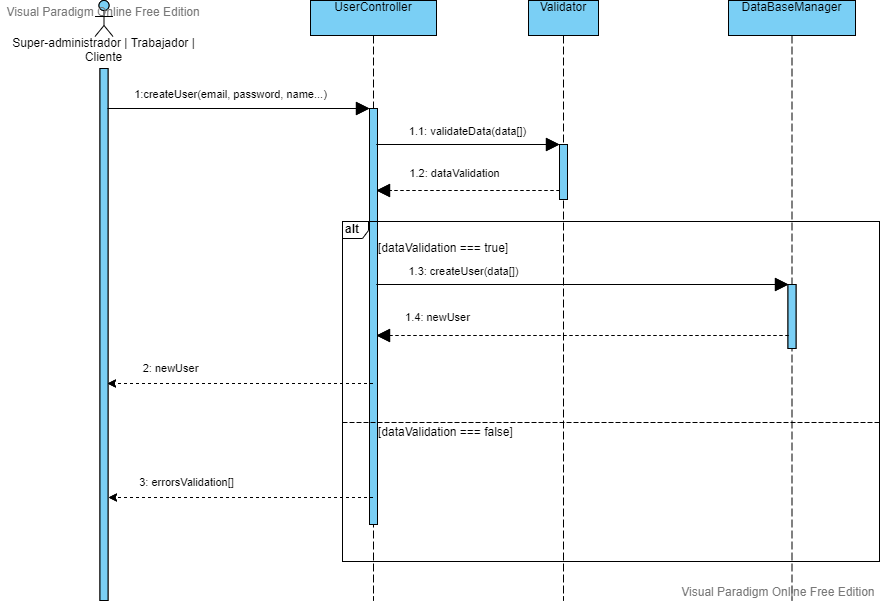
\includegraphics[scale=0.42]{images/Alta_Usuario.png}
  \caption{DS: Alta de cliente, trabajador o super-administrador.}
  \label{DS1}
\end{figure}

\begin{figure}[H]
  \centering
  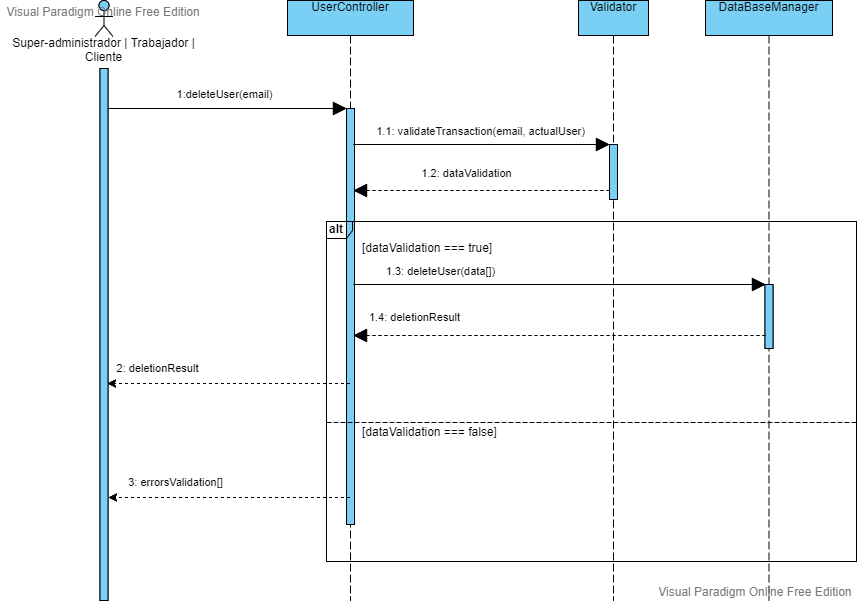
\includegraphics[scale=0.42]{images/Baja_Usuario.png}
  \caption{DS: Baja de cliente, trabajador o super-administrador.}
  \label{DS1}
\end{figure}

\begin{figure}[H]
  \centering
  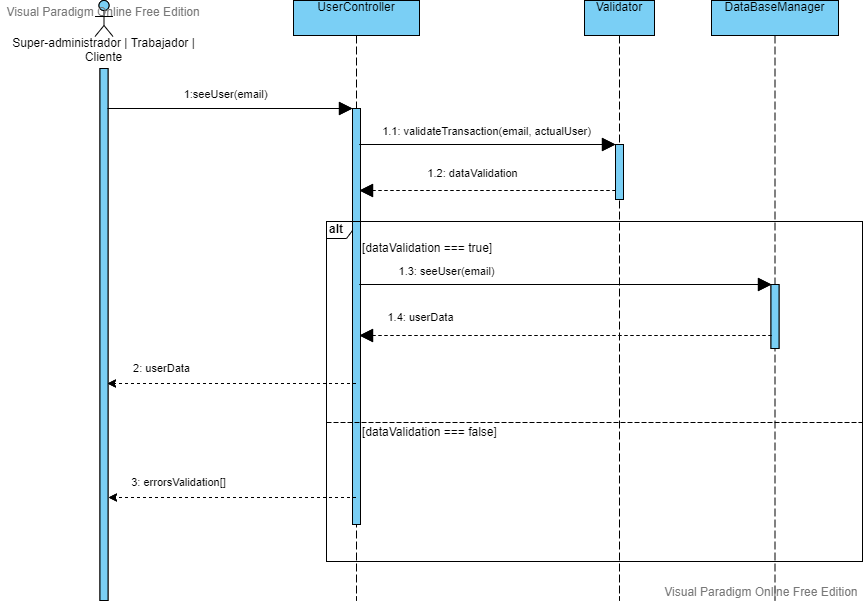
\includegraphics[scale=0.42]{images/Consultar_Datos_Usuario.png}
  \caption{DS: Consultar datos de cliente, trabajador o super-administrador.}
  \label{DS1}
\end{figure}

\begin{figure}[H]
  \centering
  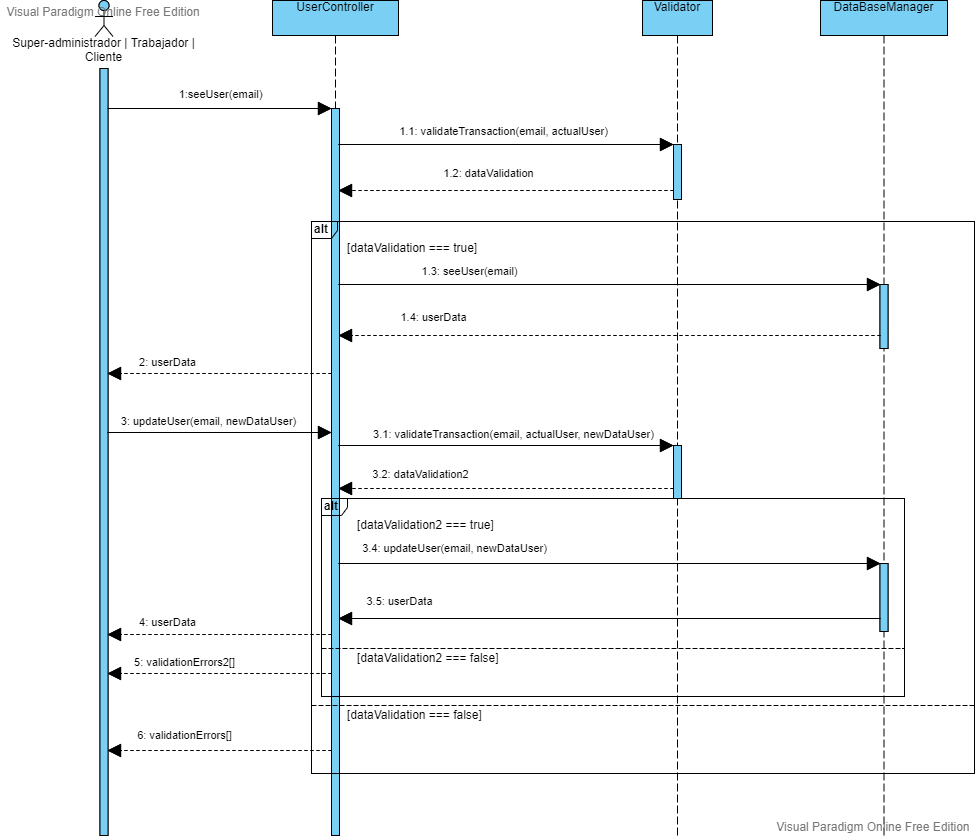
\includegraphics[scale=0.38]{images/Modificar_Datos_Usuario.png}
  \caption{DS: Modificar datos de cliente, trabajador o super-administrador.}
  \label{DS1}
\end{figure}

\begin{figure}[H]
  \centering
  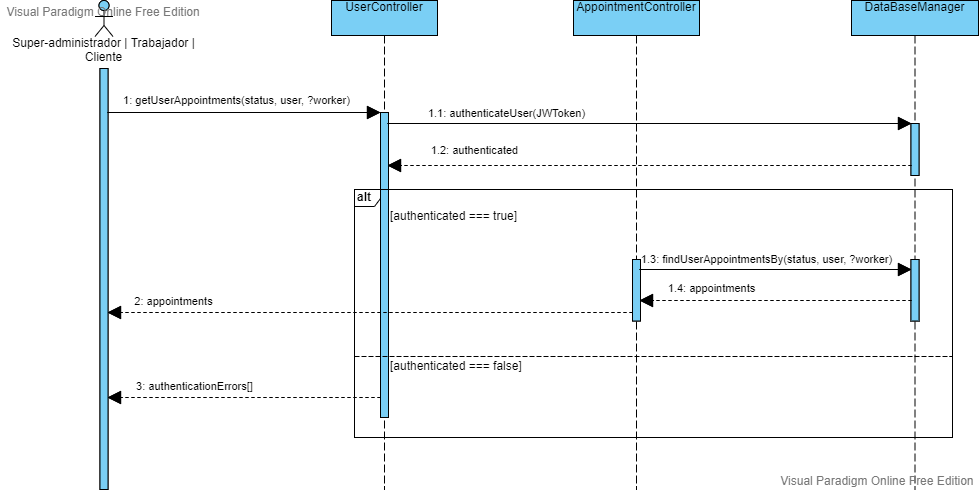
\includegraphics[scale=0.38]{images/Consultar_citas.png}
  \caption{DS: Consultar citas por cliente, trabajador o super-administrador.}
  \label{DS1}
\end{figure}

\begin{figure}[H]
  \centering
  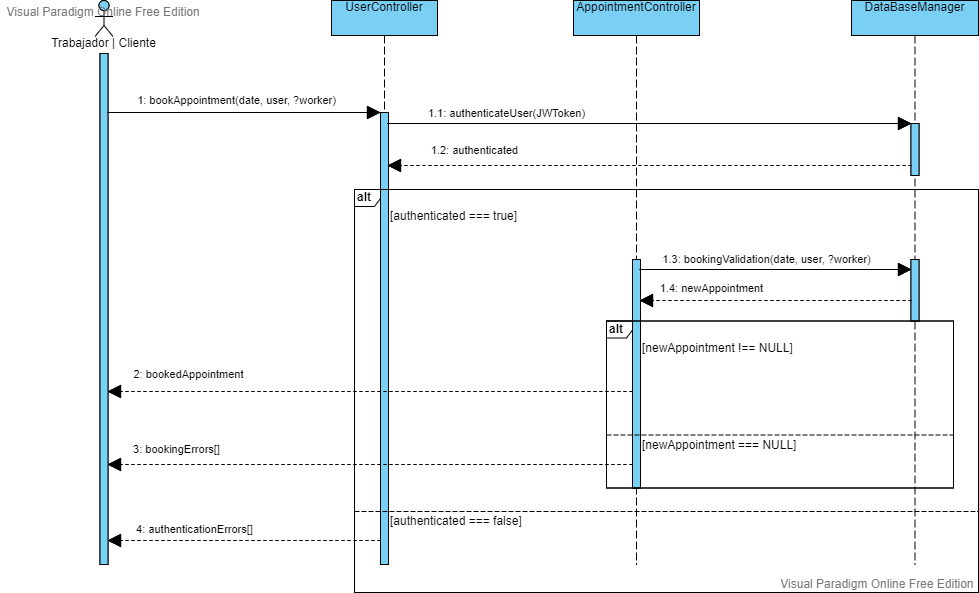
\includegraphics[scale=0.36]{images/Rerservar_cita.png}
  \caption{DS: Reserva de cita por cliente o trabajador.}
  \label{DS1}
\end{figure}

\begin{figure}[H]
  \centering
  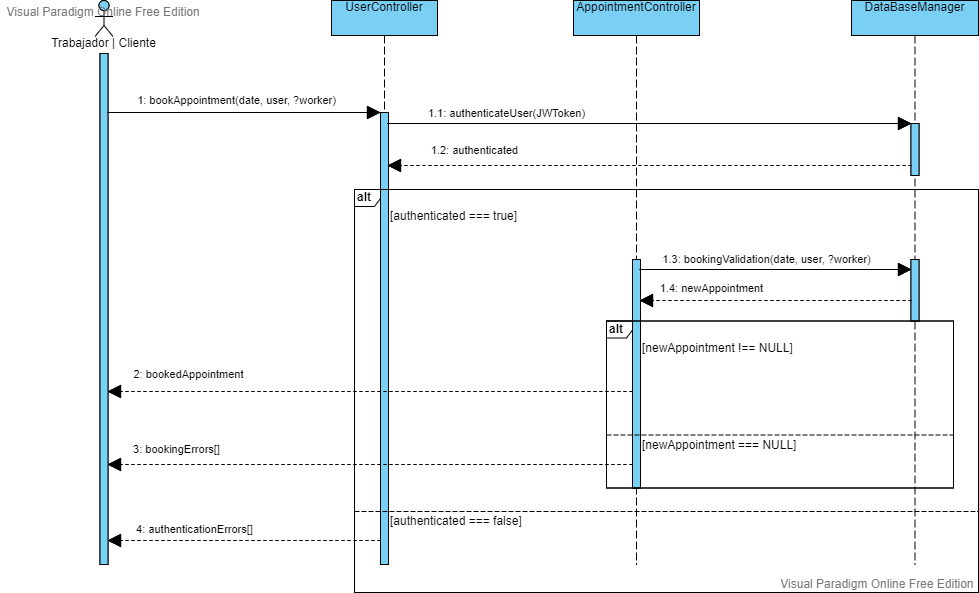
\includegraphics[scale=0.36]{images/Rerservar_cita.png}
  \caption{DS: Cancelación de cita por cliente o trabajador.}
  \label{DS1}
\end{figure}


\begin{figure}[H]
  \centering
  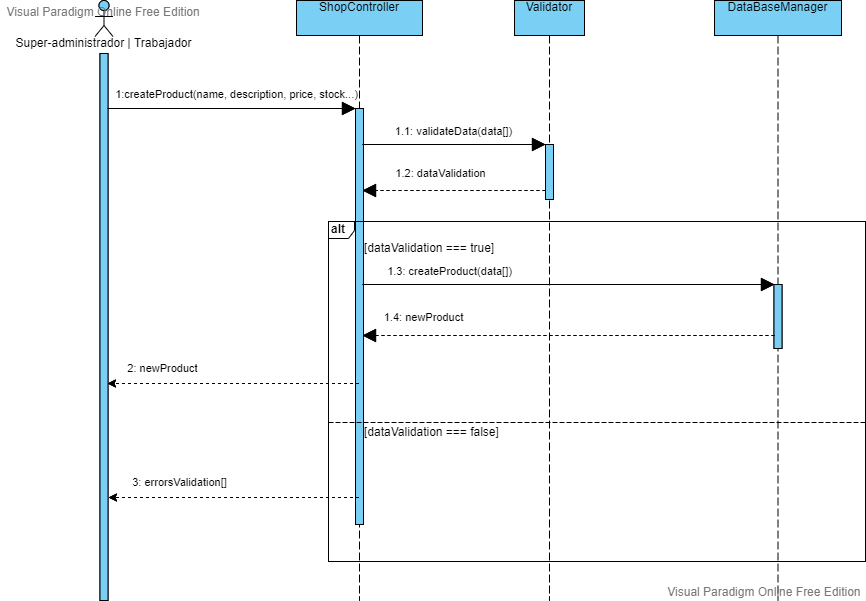
\includegraphics[scale=0.38]{images/Alta_Producto.png}
  \caption{DS: Alta de producto para venta online por trabajador o super-administrador.}
  \label{DS1}
\end{figure}

\begin{figure}[H]
  \centering
  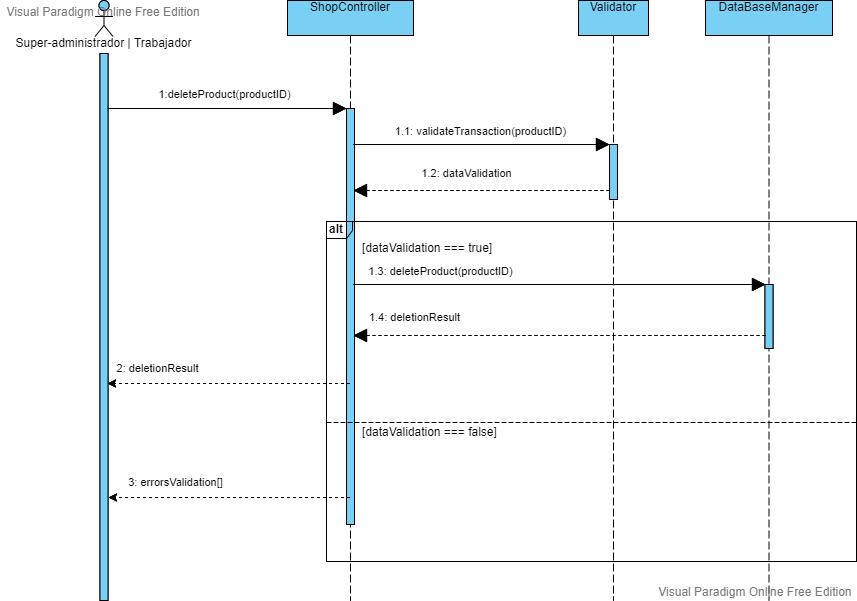
\includegraphics[scale=0.38]{images/Baja_Producto.png}
  \caption{DS: Baja de producto para venta online por trabajador o super-administrador.}
  \label{DS1}
\end{figure}

\begin{figure}[H]
  \centering
  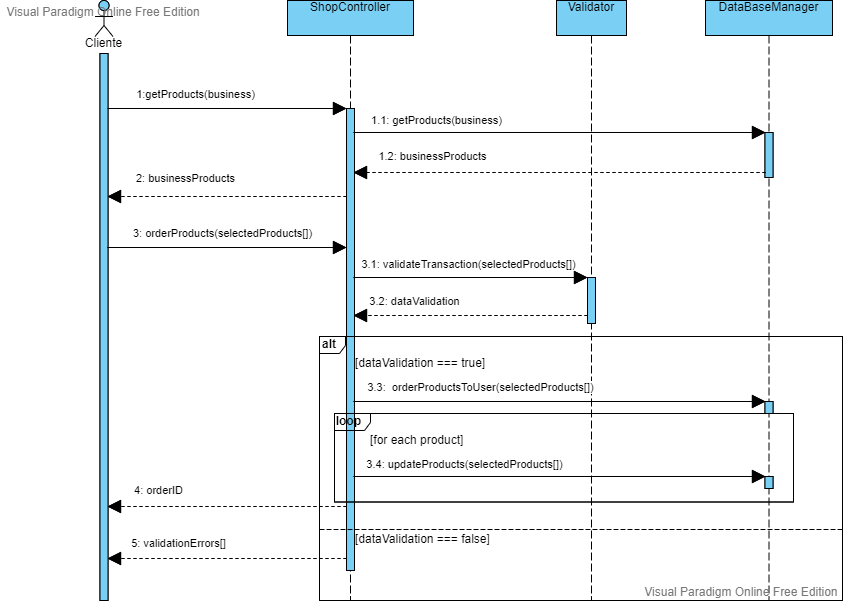
\includegraphics[scale=0.42]{images/Realizar_Pedido.png}
  \caption{DS: Realizar pedido de productos por cliente.}
  \label{DS1}
\end{figure}

\begin{figure}[H]
  \centering
  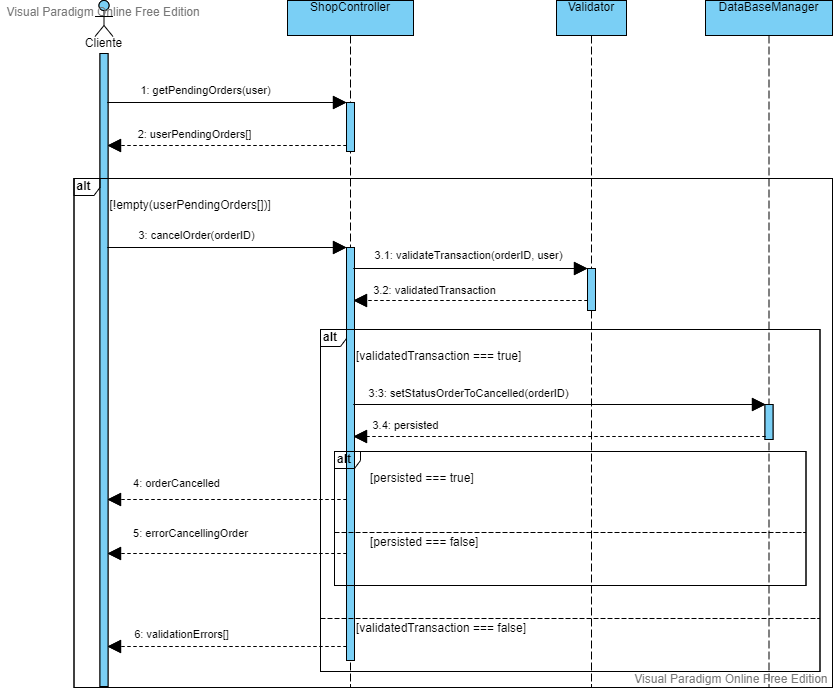
\includegraphics[scale=0.42]{images/Cancelar_Pedido.png}
  \caption{DS: Cancelar pedido por cliente.}
  \label{DS1}
\end{figure}

\begin{figure}[H]
  \centering
  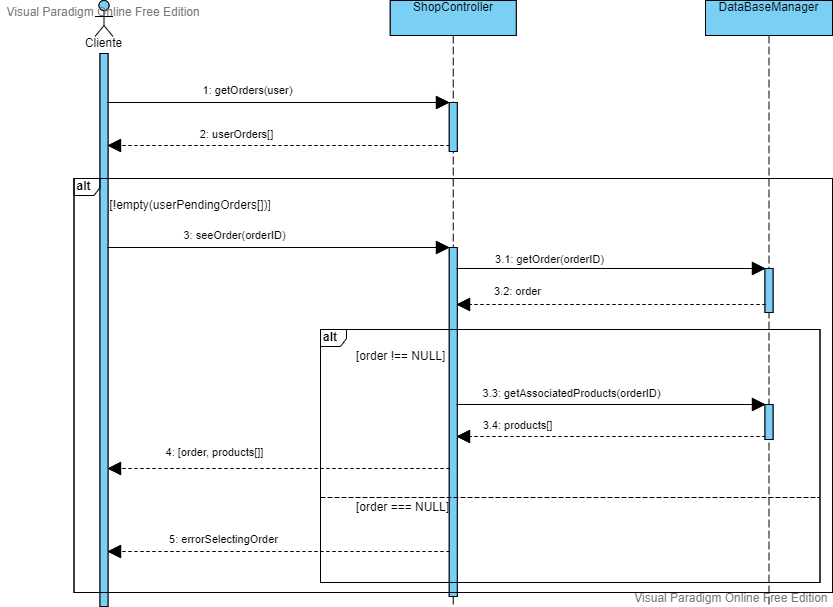
\includegraphics[scale=0.42]{images/Consultar_Pedido.png}
  \caption{DS: Consultar pedido de productos por cliente.}
  \label{DS1}
\end{figure}



